\documentclass[11pt,a4paper]{article}
\usepackage[T1]{fontenc}
\usepackage[utf8]{inputenc}
\usepackage{lmodern}
\usepackage[english]{babel}
\usepackage{amsmath,amssymb,geometry,enumitem,tikz}
\usetikzlibrary{arrows.meta,patterns}
\geometry{margin=24mm}
\setlength{\parindent}{0pt}
\setlength{\parskip}{6pt}
\title{Linear Optimization (311.160)\\Exercise sheet 2}
\author{Raphael Bleier}
\date{}
\begin{document}
\maketitle

The course workflow says to solve the exercises on the sheet, but not the classroom task. I therefore leave classroom task 2.1 out of this PDF.

\section*{Exercise 2.1: standard form, feasibility and boundedness}

I use the lecture's standard form
\[
\max\;c^{\mathsf T}x\quad\text{subject to}\quad Ax=b,\quad x\geq0.
\]
For the original problem, introduce a slack variable for each inequality:
\begin{align*}
\max\quad &2x_1+x_2\\
\text{subject to}\quad
&2x_1-x_2+s_1=12,\\
&x_1+s_2=8,\\
&x_1,x_2,s_1,s_2\geq0.
\end{align*}
Thus, with $x=(x_1,x_2,s_1,s_2)^{\mathsf T}$,
\[
 c=\begin{pmatrix}2\\1\\0\\0\end{pmatrix},\qquad
 b=\begin{pmatrix}12\\8\end{pmatrix},\qquad
 A=\begin{pmatrix}2&-1&1&0\\1&0&0&1\end{pmatrix}.
\]
The point $(x_1,x_2,s_1,s_2)=(0,0,12,8)$ is feasible. The LP is unbounded: for any $t\geq0$, $(x_1,x_2)=(0,t)$ satisfies the original constraints and has objective value $t$. Hence the objective can be made arbitrarily large.

\section*{Exercise 2.2: reading the graph}

The shaded region lies to the right of $x_1=3$ and above both dashed/solid boundary lines. Reading their intercepts and slopes gives
\[
2x_1+3x_2\geq12,\qquad x_1-2x_2\leq1,\qquad x_1\geq3.
\]
The objective contours in the figure have slope $-2$ and are parallel to $2x_1+x_2=\text{constant}$. Their direction of increase points up and to the right, so the LP shown is
\begin{align*}
\max\quad &2x_1+x_2\\
\text{subject to}\quad
&2x_1+3x_2\geq12,\\
&x_1-2x_2\leq1,\\
&x_1\geq3.
\end{align*}
A feasible ray is $(x_1,x_2)=(5+t,2+t/2)$ for $t\geq0$. It satisfies $x_1-2x_2=1$ and $2x_1+3x_2=16+\tfrac72t\geq12$, while the objective is $12+\tfrac52t$. The objective therefore grows without bound.

\begin{center}
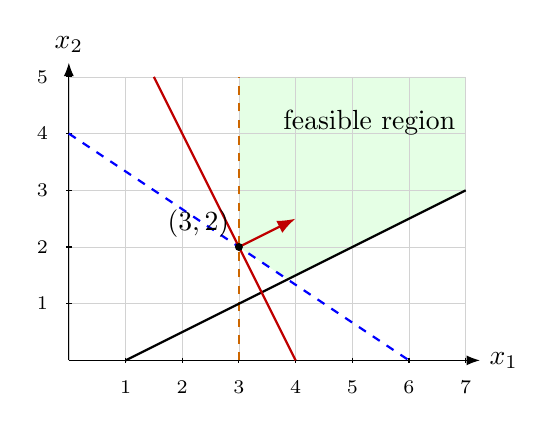
\begin{tikzpicture}[scale=0.72,>=Latex]
  \fill[green!10] (3,2) -- (3,5) -- (7,5) -- (7,3) -- (27/7,10/7) -- cycle;
  \draw[step=1,gray!35,very thin] (0,0) grid (7,5);
  \draw[->] (0,0) -- (7.25,0) node[right] {$x_1$};
  \draw[->] (0,0) -- (0,5.25) node[above] {$x_2$};
  \foreach \x in {1,...,7} \draw (\x,0.05)--(\x,-0.05) node[below=3pt] {\scriptsize\x};
  \foreach \y in {1,...,5} \draw (0.05,\y)--(-0.05,\y) node[left=3pt] {\scriptsize\y};
  \draw[orange!80!black,dashed,thick] (3,0)--(3,5);
  \draw[blue,dashed,thick] (0,4)--(6,0);
  \draw[black,thick] (1,0)--(7,3);
  \draw[red!75!black,thick] (1.5,5)--(4,0);
  \draw[->,red!75!black,thick] (3,2)--(4,2.5);
  \fill (3,2) circle (2pt) node[above left] {$(3,2)$};
  \node at (5.3,4.2) {feasible region};
\end{tikzpicture}

\smallskip
\footnotesize Dashed blue: $2x_1+3x_2=12$; black: $x_1-2x_2=1$; orange: $x_1=3$; red: objective contour.
\end{center}

\section*{Exercise 2.3: graphical solution}

The feasible region is in the first quadrant, below both resource constraints, and between $x_2=0$ and $x_2=4$. Its corner points are
\[
(0,0),\quad \left(\frac{16}{3},0\right),\quad (4,4),\quad (0,4).
\]
The two resource constraints meet at $(4,4)$, which also lies on $x_2=4$. Evaluating the objective at the corners gives
\[
\begin{array}{c|rrrr}
(x_1,x_2)&(0,0)&(16/3,0)&(4,4)&(0,4)\\\hline
3x_1+5x_2&0&16&32&20
\end{array}
\]
Thus $(x_1^*,x_2^*)=(4,4)$ and the maximum value is $32$. As a check, the constraints $3x_1+x_2\leq16$ and $x_2\leq4$ imply
\[
3x_1+5x_2=(3x_1+x_2)+4x_2\leq16+16=32,
\]
and $(4,4)$ attains this bound.

\begin{center}
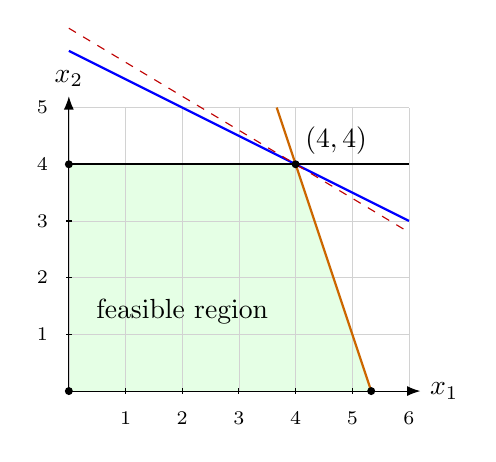
\begin{tikzpicture}[scale=0.72,>=Latex]
  \fill[green!10] (0,0)--(16/3,0)--(4,4)--(0,4)--cycle;
  \draw[step=1,gray!35,very thin] (0,0) grid (6,5);
  \draw[->] (0,0)--(6.2,0) node[right] {$x_1$};
  \draw[->] (0,0)--(0,5.2) node[above] {$x_2$};
  \foreach \x in {1,...,6} \draw (\x,0.05)--(\x,-0.05) node[below=3pt] {\scriptsize\x};
  \foreach \y in {1,...,5} \draw (0.05,\y)--(-0.05,\y) node[left=3pt] {\scriptsize\y};
  \draw[blue,thick] (0,6)--(6,3);
  \draw[orange!80!black,thick] (11/3,5)--(16/3,0);
  \draw[black,thick] (0,4)--(6,4);
  \draw[red!75!black,dashed] (0,6.4)--(6,2.8);
  \fill (0,0) circle (2pt);
  \fill (16/3,0) circle (2pt);
  \fill (4,4) circle (2pt) node[above right] {$(4,4)$};
  \fill (0,4) circle (2pt);
  \node at (2,1.4) {feasible region};
\end{tikzpicture}

\smallskip
\footnotesize Blue: $x_1+2x_2=12$; orange: $3x_1+x_2=16$; black: $x_2=4$; red dashed: objective contour.
\end{center}

\end{document}
